% The file is based on the beamer/solutions/conference-talks/
% conference-ornate-20min.en.tex template.

\documentclass{beamer}

\mode<presentation>
{
  \usetheme{Warsaw}
  \setbeamercovered{transparent}
}

\usepackage[english]{babel}
\usepackage[latin1]{inputenc}
\usepackage[T1]{fontenc}

\title
{Current Content Discovery for Business Module Teaching}

\author
{Guanyuming He}

\institute[Imperial College London]
{
  Department of Earth Science and Engineering\\
  Imperial College London
}

\date[IRP 25]
{Independent Research Project, 2025}

% If you have a file called "university-logo-filename.xxx", where xxx
% is a graphic format that can be processed by latex or pdflatex,
% resp., then you can add a logo as follows:

% \pgfdeclareimage[height=0.5cm]{university-logo}{university-logo-filename}
% \logo{\pgfuseimage{university-logo}}


% If you wish to uncover everything in a step-wise fashion, uncomment
% the following command: 

%\beamerdefaultoverlayspecification{<+->}

\begin{document}

\begin{frame}
  \titlepage
\end{frame}

\begin{frame}{Outline}
  \tableofcontents
  % You might wish to add the option [pausesections]
\end{frame}


% Structuring a talk is a difficult task and the following structure
% may not be suitable. Here are some rules that apply for this
% solution: 

% - Exactly two or three sections (other than the summary).
% - At *most* three subsections per section.
% - Talk about 30s to 2min per frame. So there should be between about
%   15 and 30 frames, all told.

% - A conference audience is likely to know very little of what you
%   are going to talk about. So *simplify*!
% - In a 20min talk, getting the main ideas across is hard
%   enough. Leave out details, even if it means being less precise than
%   you think necessary.
% - If you omit details that are vital to the proof/implementation,
%   just say so once. Everybody will be happy with that.

\section{Introduction}

\subsection{Motivation}

\begin{frame}{Business School Case Method}

  \begin{itemize}
  \item
    First institutionalized at Harvard Business School. One of the mainstream
	teaching methods.
  \item
	Christensen identifies that instructors have to conduct ``extensive
	preparation'' for it.
  \end{itemize}
\end{frame}

\begin{frame}{Past advancements in information retrieval}
  \begin{itemize}
	\item No significant improvement until the 19th century.
	\item (Wired) Morse et al.'s telegraph (1840) and Bell's telephone (1876).
	\item (Wireless) Marconi's experiments ($\sim 1900$), first radio voice
		broadcast (1906) 
	\item (Theory) Frequency modulation ($\sim 1930$).  Shannon's bits and
		entropy (1948).   
	\item (Modern) Digital computers, database systems, the Internet.
	\item (Contemporary) Web search engines. Data Science. LLMs.
\end{itemize}
\end{frame}

\subsection{Related Works}

\begin{frame}{Improvements on LLMs}
	\begin{itemize}
		\item RAG: use pretrained retriever to address hallucination.
		\item A lot others that use external knowledge to augment LLMs. Most
			are to improve question answering.
		\item Perhaps most similar to mine among them: WebGPT, whose retriever
			is not a model, but a web browser that the LLM can use.
	\end{itemize}
\end{frame}

\begin{frame}{Improvements on Search engines}
	\begin{itemize}
		\item Some use LLMs to rewrite and improve search queries.
		\item Some use LLMs to assist ranking of search results.
		\item A few use LLMs in the indexing stage for NLP tasks (e.g.\ term
			extraction, meaning filtering).
	\end{itemize}
\end{frame}

\section{Methodology}
\subsection{Design philosophy \& Architecture}
\begin{frame}{Design philosophy \& Architecture}
	\begin{itemize}
		\item Three software engineering pinciples.
		\item Modular design from the UNIX philosophy.
		\item A main pipeline and surrounding support programs (scheduling,
			search engine, GUI).
	\end{itemize}

	\begin{center}
		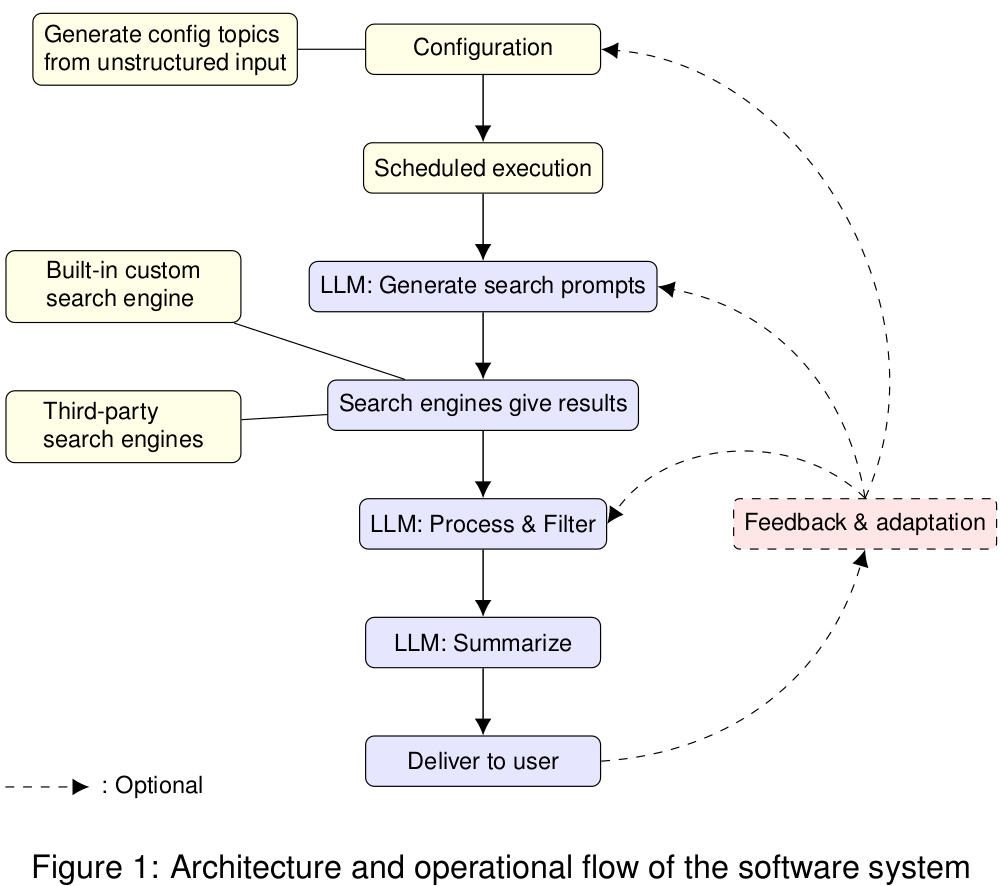
\includegraphics[height=.5\textheight]{./architecture.png}
	\end{center}

\end{frame}

\subsection{Technical plans}
\begin{frame}{Technical plans}
	\begin{itemize}
		\item Use C++ and a number of libraries to implement the custom search
			engine and supporting programs.
		\item Use Python to implement the rest programs.
		\item Use Ollama to invoke LLMs. 
		\item Use Cron to schedule tasks. Use Email for results delivery.
	\end{itemize}
\end{frame}

\section{Our Results/Contribution}
\subsection{Main Results}

\begin{frame}{Make Titles Informative.}
\end{frame}

\begin{frame}{Make Titles Informative.}
\end{frame}

\begin{frame}{Make Titles Informative.}
\end{frame}


\subsection{Comparsion with mainstream tools}

\begin{frame}{Make Titles Informative.}
\end{frame}

\begin{frame}{Make Titles Informative.}
\end{frame}

\begin{frame}{Make Titles Informative.}
\end{frame}


\section*{Summary}

\begin{frame}{Summary}

  % Keep the summary *very short*.
  \begin{itemize}
  \item
    The \alert{first main message} of your talk in one or two lines.
  \item
    The \alert{second main message} of your talk in one or two lines.
  \item
    Perhaps a \alert{third message}, but not more than that.
  \end{itemize}
  
  % The following outlook is optional.
  \vskip0pt plus.5fill
  \begin{itemize}
  \item
    Outlook
    \begin{itemize}
    \item
      Something you haven't solved.
    \item
      Something else you haven't solved.
    \end{itemize}
  \end{itemize}
\end{frame}



% All of the following is optional and typically not needed. 
\appendix
\section<presentation>*{\appendixname}
\subsection<presentation>*{For Further Reading}

\begin{frame}[allowframebreaks]
  \frametitle<presentation>{For Further Reading}
    
  \begin{thebibliography}{10}
    
  \beamertemplatebookbibitems
  % Start with overview books.

  \bibitem{Author1990}
    A.~Author.
    \newblock {\em Handbook of Everything}.
    \newblock Some Press, 1990.
 
    
  \beamertemplatearticlebibitems
  % Followed by interesting articles. Keep the list short. 

  \bibitem{Someone2000}
    S.~Someone.
    \newblock On this and that.
    \newblock {\em Journal of This and That}, 2(1):50--100,
    2000.
  \end{thebibliography}
\end{frame}

\end{document}


